\subsection*{1.}
The process is Markov, since knowing $X_t$ tells us the same amount of information about $X_{t+1}$ as knowing $(X_j)_{j=0}^t$. The transition probability can be calculated with the density transform. 
\begin{gather*}
X_{t+1}=y=(aX_t+b+\epsilon_{t+1})^3 \Longrightarrow \epsilon_{t+1}=y^{1/3}-aX_t-b ~~~~~ \frac{\partial}{\partial y}= \frac{y^{-2/3}}{3}    
\end{gather*}
So the conditional density can be written as follows with the density of $\epsilon_{t+1} \sim f_\epsilon$
\begin{gather*}
    p(y|X_t=x)=f_{\epsilon}(y^{1/3}-ax-b)\frac{y^{-2/3}}{3} \bigg \rvert_{x=X_{t}}
\end{gather*}
With the transition density, we can compute the conditional expectations
\begin{gather*}
    \cE{X_{t+1}}{X_t}=\int_{\R}y p(y|x)\dy\dummy{x=X_t}=\int_{\R}yf_{\epsilon}(y^{1/3}-ax-b)\frac{y^{-2/3}}{3}\dy\dummy{x=X_t}=\\
    \int_{\R}\frac{y^{1/3}}{3}\frac{1}{\sqrt{2\pi}\sigma}\exp-\frac{1}{2}\left(
    -\frac{y^{1/3}-ax-b-\mu}{\sigma}  \right)^2 \dy= \int_{\R} 3 \frac{z^3}{3}f_{\tilde{\epsilon}}(z)\dz = \E{\tilde{\epsilon}^3}=(aX_t+b+\mu)^3+3(aX_t+b+\mu)\sigma^2 
\end{gather*}
where we used the substitution $y=z^3$ with $dy=3z^2dz$, and denote $\tilde{\epsilon}\sim\gauss{aX_t+b+\mu}{\sigma^2}$. In the last equality we used the fact that the third moment of a normal variable equals to $\E{X^3}=\mu^3+3\mu\sigma^2$ if $X\sim\gauss{\mu}{\sigma^2}$
\begin{gather*}
    \cE{X_{t+1}^2}{X_t}=\int_{\R}y^2 p(y|x)\dy\dummy{x=X_t}= \int_{\R}y^2f_{\epsilon}(y^{1/3}-ax-b)\frac{y^{-2/3}}{3}\dy\dummy{x=X_t}=\\
    \int_{\R}\frac{y^{4/3}}{3}f_{\epsilon}(y^{1/3}-ax-b)\dy\dummy{x=X_t}=
    \int_{\R}\frac{z^{4}}{3}f_{\tilde{\epsilon}}(z)3z^2\dz = \E{\tilde{\epsilon}^6}
\end{gather*}
So the result is the sixth moment of the normal variable with mean $aX_t+b+\mu$ and variance $\sigma^2$.

\subsection*{2.}
\begin{itemize}
    \item $E[X_{t+1}|\mathcal{F}_{t}]$
    %\begin{gather*}
    %    E[X_{t+1}|\mathcal{F}_{t}] = E[X_{t+1}|X_{0},...,X_{t}] = E[X_{t+1}|X_{t}] = E[X_{t+1}|X_{t}=x_{t}] =\\ =x_{1}(p_{(x_{t},y_{1}),(x_{1},y_{1})}+p_{(x_{t},y_{1}),(x_{1},y_{2})}+p_{(x_{t},y_{2}),(x_{1},y_{1})}+p_{(x_{t},y_{2}),(x_{1},y_{2})})\\
    %    + x_{2}(p_{(x_{t},y_{1}),(x_{2},y_{1})}+p_{(x_{t},y_{1}),(x_{2},y_{2})}+p_{(x_{t},y_{2}),(x_{2},y_{1})}+p_{(x_{t},y_{2}),(x_{2},y_{2})})
    %\end{gather*}
    %Where $x_{t}$ can be either $x_{1}$ or $x_{2}$.
    \begin{gather*}
        E[X_{t+1}|\mathcal{F}_{t}] = E[X_{t+1}|(X_{0},Y_{0}),...,(Y_{t},X_{t})] = E[X_{t+1}|(X_{t},Y_{t})] =\\
        =x_{1}(p_{(x_{t},y_{t}),(x_{1},y_{1})}+p_{(x_{t},y_{t}),(x_{1},y_{2})})+x_{2}(p_{(x_{t},y_{t}),(x_{2},y_{1})}+p_{(x_{t},y_{t}),(x_{2},y_{2})})
    \end{gather*}
    Where $(x_t,y_t)$ can take four values: $(x_1,y_1)$, $(x_1,y_2)$, $(x_2,y_1)$ and $(x_2,y_2)$.\\
Remark: We can summarize the above calculations using the Kolmogorov equations. For example: 

$E[X_{t+1}|\mathcal{F}_{t}] = \Pi^T_{(x_i, y_j)} \begin{pmatrix}
x_1 \\ x_1 \\ x_2 \\ x_2 
\end{pmatrix}$

 Where $\Pi^T_{(x_i, y_j)}$  is the row of the transition matrix to the power $T$ corresponding to the state $(x_i,y_j)$.

    \item $E[X_{t+1}|\mathcal{F}_{t+1}]$
    \begin{gather*}
        E[X_{t+1}|\mathcal{F}_{t+1}] = E[X_{t+1}|(X_{0},Y_{0}),...,(X_{t+1},Y_{t+1})] = E[X_{t+1}|(X_{t+1},Y_{t+1})] = x_{t+1}
    \end{gather*}
    Where $x_{t+1}$ can be either $x_{1}$ or $x_{2}$.
    \item $E[X_{t+1}|\mathcal{F}_{t-1}]$
    %\begin{gather*}
     %   E[X_{t+1}|\mathcal{F}_{t-1}] = E[X_{t+1}|X_{0},...,X_{t-1}] = E[X_{t+1}|X_{t-1}] = E[X_{t+1}|X_{t-1}=x_{t-1}] =\\
      %  =x_{1}(p_{(x_{t-1},y_{1})(x_{1},y_{1})}(p_{(x_{1},y_{1})(x_{1},y_{1})}+p_{(x_{1},y_{1})(x_{1},y_{2})})+p_{(x_{t-1},y_{1})(x_{1},y_{2})}(p_{(x_{1},y_{2})(x_{1},y_{1})}+p_{(x_{1},y_{2})(x_{1},y_{2})})+\\
       % +p_{(x_{t-1},y_{1})(x_{2},y_{1})}(p_{(x_{2},y_{1})(x_{1},y_{1})}+p_{(x_{2},y_{1})(x_{1},y_{2})})+p_{(x_{t-1},y_{1})(x_{2},y_{2})}(p_{(x_{2},y_{2})(x_{1},y_{1})}+p_{(x_{2},y_{2})(x_{1},y_{2})})+\\
        %+p_{(x_{t-1},y_{2})(x_{1},y_{1})}(p_{(x_{1},y_{1})(x_{1},y_{1})}+p_{(x_{1},y_{1})(x_{1},y_{2})})+p_{(x_{t-1},y_{2})(x_{1},y_{2})}(p_{(x_{1},y_{2})(x_{1},y_{1})}+p_{(x_{1},y_{2})(x_{1},y_{2})})+\\
    %    +p_{(x_{t-1},y_{2})(x_{2},y_{1})}(p_{(x_{2},y_{1})(x_{1},y_{1})}+p_{(x_{2},y_{1})(x_{1},y_{2})})+p_{(x_{t-1},y_{2})(x_{2},y_{2})}(p_{(x_{2},y_{2})(x_{1},y_{1})}+p_{(x_{2},y_{2})(x_{1},y_{2})}))+\\
     %   +x_{2}(p_{(x_{t-1},y_{1})(x_{1},y_{1})}(p_{(x_{1},y_{1})(x_{2},y_{1})}+p_{(x_{1},y_{1})(x_{2},y_{2})})+p_{(x_{t-1},y_{1})(x_{1},y_{2})}(p_{(x_{1},y_{2})(x_{2},y_{1})}+p_{(x_{1},y_{2})(x_{2},y_{2})})+\\
    %    +p_{(x_{t-1},y_{1})(x_{2},y_{1})}(p_{(x_{2},y_{1})(x_{2},y_{1})}+p_{(x_{2},y_{1})(x_{2},y_{2})})+p_{(x_{t-1},y_{1})(x_{2},y_{2})}(p_{(x_{2},y_{2})(x_{2},y_{1})}+p_{(x_{2},y_{2})(x_{2},y_{2})})+\\
     %   +p_{(x_{t-1},y_{2})(x_{1},y_{1})}(p_{(x_{1},y_{1})(x_{2},y_{1})}+p_{(x_{1},y_{1})(x_{2},y_{2})})+p_{(x_{t-1},y_{2})(x_{1},y_{2})}(p_{(x_{1},y_{2})(x_{2},y_{1})}+p_{(x_{1},y_{2})(x_{2},y_{2})})+\\
      %  +p_{(x_{t-1},y_{2})(x_{2},y_{1})}(p_{(x_{2},y_{1})(x_{2},y_{1})}+p_{(x_{2},y_{1})(x_{2},y_{2})})+p_{(x_{t-1},y_{2})(x_{2},y_{2})}(p_{(x_{2},y_{2})(x_{2},y_{1})}+p_{(x_{2},y_{2})(x_{2},y_{2})}))
    %\end{gather*}
    %Where $x_{t-1}$ can be either $x_{1}$ or $x_{2}$.
   \begin{gather*}
    E[X_{t+1}|\mathcal{F}_{t-1}] = E[X_{t+1}|(X_{0},Y_{0}),...,(X_{t-1},Y_{t-1})] = E[X_{t+1}|(X_{t-1},Y_{t-1})] = \\
    =x_{1}(p_{(x_{t-1},y_{t-1})(x_{1},y_{1})}(p_{(x_{1},y_{1})(x_{1},y_{1})}+p_{(x_{1},y_{1})(x_{1},y_{2})})+p_{(x_{t-1},y_{t-1})(x_{1},y_{2})}(p_{(x_{1},y_{2})(x_{1},y_{1})}+p_{(x_{1},y_{2})(x_{1},y_{2})})+\\
    +p_{(x_{t-1},y_{t-1})(x_{2},y_{1})}(p_{(x_{2},y_{1})(x_{1},y_{1})}+p_{(x_{2},y_{1})(x_{1},y_{2})})+p_{(x_{t-1},y_{t-1})(x_{2},y_{2})}(p_{(x_{2},y_{2})(x_{1},y_{1})}+p_{(x_{2},y_{2})(x_{1},y_{2})})+\\
    +x_{2}(p_{(x_{t-1},y_{t-1})(x_{1},y_{1})}(p_{(x_{1},y_{1})(x_{2},y_{1})}+p_{(x_{1},y_{1})(x_{2},y_{2})})+p_{(x_{t-1},y_{t-1})(x_{1},y_{2})}(p_{(x_{1},y_{2})(x_{2},y_{1})}+p_{(x_{1},y_{2})(x_{2},y_{2})})+\\
    +p_{(x_{t-1},y_{t-1})(x_{2},y_{1})}(p_{(x_{2},y_{1})(x_{2},y_{1})}+p_{(x_{2},y_{1})(x_{2},y_{2})})+p_{(x_{t-1},y_{1})(x_{2},y_{2})}(p_{(x_{2},y_{2})(x_{2},y_{1})}+p_{(x_{2},y_{2})(x_{2},y_{2})}))
    \end{gather*}
    Where $(x_t,y_t)$ can take four values: $(x_1,y_1)$, $(x_1,y_2)$, $(x_2,y_1)$ and $(x_2,y_2)$. \\
    %$E[X_{t+1}|Y_{t}]$
    %\begin{gather*}
        %E[X_{t+1}|Y_{t}] = E[X_{t+1}|Y_{t} = y_{t}] =\\
        %= x_{1}(p_{(x_{1},y_{t}),(x_{1},y_{1})}+p_{(x_{1},y_{t}),(x_{1},y_{2})}+p_{(x_{2},y_{t}),(x_{1},y_{1})}+p_{(x_{2},y_{t}),(x_{1},y_{2})})\\
        %+ x_{2}(p_{(x_{1},y_{t}),(x_{2},y_{1})}+p_{(x_{1},y_{t}),(x_{2},y_{2})}+p_{(x_{2},y_{t}),(x_{2},y_{1})}+p_{(x_{2},y_{t}),(x_{2},y_{2})})
    %\end{gather*}
    %Where $y_{t}$ can be either $y_{1}$ or $y_{2}$. 

\item     
Let $\Pi^T_{(x_i, y_j)}$ the row of the transition matrix to the power $T$ corresponding to the state $(x_i,y_j)$. Let $p_0$ the initial distibution of the Markov chain.\\
Then $P(X_t = x_i, Y_t = y_j ) = \Pi^t_{(x_i,y_j)} p_0$. Also,
\begin{gather*}
    P(Y_t = y_j) = P(X_t = x_1, Y_t = y_j) + P(X_t= X_2, Y_t=y_j)
    =\Pi^t_{(x_1,y_j)} p_0 + \Pi^t_{(x_2,y_j)} p_0
\end{gather*}
And,
\begin{gather}
    P(X_t = x_i|Y_t = y_j) = \frac{P(X_t = x_i, Y_t = y_j )}{P(Y_t = y_j)} = \frac{\Pi^t_{(x_i,y_j)} p_0}{\Pi^t_{(x_1,y_j)} p_0 + \Pi^t_{(x_2,y_j)} p_0} 
\end{gather}

\begin{itemize}
    \item $E[X_{t+1}|Y_t]$
    \begin{gather*}
    E[X_{t+1}|Y_t] = \sum_{i=1,2} x_i P(X_{t+1} = x_i | Y_t)
    = \sum_{i=1,2} x_i \sum_{j=1,2} P(X_{t+1} = x_i, X_t = x_j | Y_t)\\
    %=\sum_{i=1,2} x_i \sum_{j=1,2} P(X_{t+1} = x_i|X_t = x_j, Y_t) P(X_t = x_j|Y_t)\\
    %=\sum_{i=1,2}\sum_{j=1,2} x_i P(X_{t+1} = x_i|X_t = x_j, Y_t) P(X_t = x_j|Y_t)\\
    %=\sum_{j=1,2}\sum_{i=1,2} x_i P(X_{t+1} = x_i|X_t = x_j, Y_t) P(X_t = x_j|Y_t)\\
    %=\sum_{j=1,2} P(X_t = x_j|Y_t) \sum_{i=1,2} x_i P(X_{t+1} = x_i|X_t = x_j, Y_t)\\
    =\sum_{j=1,2} P(X_t = x_j|Y_t) E[X_{t+1}|(X_t,Y_t)=(x_j,y_t)]\\
    =\sum_{j=1,2} \frac{\Pi^t_{(x_j,y_t)} p_0}{\Pi^t_{(x_1,y_t)} p_0 + \Pi^t_{(x_2,y_t)} p_0}  E[X_{t+1}|(X_t,Y_t)=(x_j,y_t)]
    \end{gather*}
    Where $E[X_{t+1}|(X_t,Y_t)=(x_j,y_t)]$ can be calculated using the first bullet point.
    
    \item $E[X_{t+1}|Y_{t-1}]$\\
    Similarly to $E[X_{t+1}|Y_t]$,
    \begin{gather*}
    E[X_{t+1}|Y_{t-1}]=\sum_{j=1,2} P(X_{t+1} = x_j|Y_{t-1}) E[X_{t+1}|(X_{t-1},Y_{t-1})=(x_j,y_t)]\\
    =\sum_{j=1,2} \frac{\Pi^{t+1}_{(x_j,y_t)} p_0}{\Pi^{t+1}_{(x_1,y_t)} p_0 + \Pi^{t+1}_{(x_2,y_t)} p_0}  E[X_{t+1}|(X_{t-1},Y_{t-1})=(x_j,y_t)]
    \end{gather*}
\end{itemize}

    \item $E[X_{t+1}|Y_{t+1}]$
    \begin{gather*}
        E[X_{t+1}|Y_{t+1}] = E[X_{t+1}|Y_{t+1}=y_{t+1}]=\\
        = x_{1}(p_{(x_{1},y_{1}),(x_{1},y_{t+1})}+p_{(x_{1},y_{2}),(x_{1},y_{t+1})}+p_{(x_{2},y_{1}),(x_{1},y_{t+1})}+p_{(x_{2},y_{2}),(x_{1},y_{t+1})})\\
        + x_{2}(p_{(x_{1},y_{1}),(x_{2},y_{t+1})}+p_{(x_{1},y_{2}),(x_{2},y_{t+1})}+p_{(x_{2},y_{1}),(x_{2},y_{t+1})}+p_{(x_{2},y_{2}),(x_{2},y_{t+1})})        
    \end{gather*}
    Where $y_{t+1}$ can be either $y_{1}$ or $y_{2}$.
    %\item $E[X_{t+1}|Y_{t-1}]$
    %\begin{gather*}
        %E[X_{t+1}|Y_{t-1}] = E[X_{t+1}|Y_{t-1}=y_{t-1}]=\\
        %=x_{1}(p_{(x_{1},y_{t-1})(x_{1},y_{1})}(p_{(x_{1},y_{1})(x_{1},y_{1})}+p_{(x_{1},y_{1})(x_{1},y_{2})})+p_{(x_{1},y_{t-1})(x_{1},y_{2})}(p_{(x_{1},y_{2})(x_{1},y_{1})}+p_{(x_{1},y_{2})(x_{1},y_{2})})+\\
        %+p_{(x_{1},y_{t-1})(x_{2},y_{1})}(p_{(x_{2},y_{1})(x_{1},y_{1})}+p_{(x_{2},y_{1})(x_{1},y_{2})})+p_{(x_{1},y_{t-1})(x_{2},y_{2})}(p_{(x_{2},y_{2})(x_{1},y_{1})}+p_{(x_{2},y_{2})(x_{1},y_{2})})+\\
        %+p_{(x_{2},y_{t-1})(x_{1},y_{1})}(p_{(x_{1},y_{1})(x_{1},y_{1})}+p_{(x_{1},y_{1})(x_{1},y_{2})})+p_{(x_{2},y_{t-1})(x_{1},y_{2})}(p_{(x_{1},y_{2})(x_{1},y_{1})}+p_{(x_{1},y_{2})(x_{1},y_{2})})+\\
        %+p_{(x_{2},y_{t-1})(x_{2},y_{1})}(p_{(x_{2},y_{1})(x_{1},y_{1})}+p_{(x_{2},y_{1})(x_{1},y_{2})})+p_{(x_{2},y_{t-1})(x_{2},y_{2})}(p_{(x_{2},y_{2})(x_{1},y_{1})}+p_{(x_{2},y_{2})(x_{1},y_{2})}))+\\
        %+x_{2}(p_{(x_{1},y_{t-1})(x_{1},y_{1})}(p_{(x_{1},y_{1})(x_{2},y_{1})}+p_{(x_{1},y_{1})(x_{2},y_{2})})+p_{(x_{1},y_{t-1})(x_{1},y_{2})}(p_{(x_{1},y_{2})(x_{2},y_{1})}+p_{(x_{1},y_{2})(x_{2},y_{2})})+\\
        %+p_{(x_{1},y_{t-1})(x_{2},y_{1})}(p_{(x_{2},y_{1})(x_{2},y_{1})}+p_{(x_{2},y_{1})(x_{2},y_{2})})+p_{(x_{1},y_{t-1})(x_{2},y_{2})}(p_{(x_{2},y_{2})(x_{2},y_{1})}+p_{(x_{2},y_{2})(x_{2},y_{2})})+\\
        %+p_{(x_{2},y_{t-1})(x_{1},y_{1})}(p_{(x_{1},y_{1})(x_{2},y_{1})}+p_{(x_{1},y_{1})(x_{2},y_{2})})+p_{(x_{2},y_{t-1})(x_{1},y_{2})}(p_{(x_{1},y_{2})(x_{2},y_{1})}+p_{(x_{1},y_{2})(x_{2},y_{2})})+\\
        %+p_{(x_{2},y_{t-1})(x_{2},y_{1})}(p_{(x_{2},y_{1})(x_{2},y_{1})}+p_{(x_{2},y_{1})(x_{2},y_{2})})+p_{(x_{2},y_{t-1})(x_{2},y_{2})}(p_{(x_{2},y_{2})(x_{2},y_{1})}+p_{(x_{2},y_{2})(x_{2},y_{2})}))
    %\end{gather*}
    %Where $y_{t-1}$ can be either $y_{1}$ or $y_{2}$.
    


\end{itemize}
\subsection*{3.}
a)

transition matrix: 
$\begin{pmatrix}
2/3 & 1/3 \\
1/3 & 2/3
\end{pmatrix} 
=
\begin{pmatrix}
-1 & 1 \\
1 & 1
\end{pmatrix}
\begin{pmatrix}
1/3 & 0 \\
0 & 1 
\end{pmatrix}
\begin{pmatrix}
-1/2 &1/2 \\
1/2 & 1/2
\end{pmatrix}$

\begin{gather*}
    \E{X_T^3+X_{T-1}^5 | X_1=x_1} =\E{X_T^3| X_1=x_1} + \E{X_{T-1}^5| X_1=x_1} = (\Pi^{T-1} x^3 + \Pi^{T-2} x^5) \begin{pmatrix}
    1 \\ 0
    \end{pmatrix} = 
\end{gather*}

$\Pi^{T-1}= 
\begin{pmatrix}
-1 & 1 \\
1 & 1
\end{pmatrix}
\begin{pmatrix}
\frac{1}{3} & 0 \\
0 & 1 
\end{pmatrix}^{T-1}
\begin{pmatrix}
-\frac{1}{2} & \frac{1}{2} \\
\frac{1}{2} & \frac{1}{2}
\end{pmatrix}=
\begin{pmatrix}
-1 & 1 \\
1 & 1
\end{pmatrix}
\begin{pmatrix}
\frac{1}{3}^{T-1} & 0 \\
0 & 1^{T-1} 
\end{pmatrix}
\begin{pmatrix}
-\frac{1}{2} &\frac{1}{2} \\
\frac{1}{2} & \frac{1}{2}
\end{pmatrix}=
\begin{pmatrix}
-\frac{1}{2} \cdot\frac{1}{3}^{T-1} +\frac{1}{2} & \frac{1}{2} \cdot\frac{1}{3}^{T-1} +\frac{1}{2} \\
-\frac{1}{2} \cdot\frac{1}{3}^{T-1} +\frac{1}{2} & \frac{1}{2} \cdot\frac{1}{3}^{T-1} +\frac{1}{2}
\end{pmatrix} $

Similarly, 

$\Pi^{T-2}=
\begin{pmatrix}
-\frac{1}{2} \cdot\frac{1}{3}^{T-2} +\frac{1}{2} & \frac{1}{2} \cdot\frac{1}{3}^{T-2} +\frac{1}{2} \\
-\frac{1}{2} \cdot\frac{1}{3}^{T-2} +\frac{1}{2} & \frac{1}{2} \cdot\frac{1}{3}^{T-2} +\frac{1}{2}
\end{pmatrix} $
\begin{gather*}
\left(\begin{pmatrix}
-\frac{1}{2} \cdot\frac{1}{3}^{T-1} +\frac{1}{2} & \frac{1}{2} \cdot\frac{1}{3}^{T-1} +\frac{1}{2} \\
-\frac{1}{2} \cdot\frac{1}{3}^{T-1} +\frac{1}{2} & \frac{1}{2} \cdot\frac{1}{3}^{T-1} +\frac{1}{2}
\end{pmatrix}
\begin{pmatrix}
x_1^3 \\
x_2^3 
\end{pmatrix}+ 
\begin{pmatrix}
-\frac{1}{2} \cdot\frac{1}{3}^{T-2} +\frac{1}{2} & \frac{1}{2} \cdot\frac{1}{3}^{T-2} +\frac{1}{2} \\
-\frac{1}{2} \cdot\frac{1}{3}^{T-2} +\frac{1}{2} & \frac{1}{2} \cdot\frac{1}{3}^{T-2} +\frac{1}{2}
\end{pmatrix}
\begin{pmatrix}
x_1^5 \\
x_2^5 
\end{pmatrix}\right)\begin{pmatrix}
    1 \\ 0
    \end{pmatrix} =\\
-\frac{1}{2} \cdot\frac{1}{3}^{T-1} +\frac{1}{2} x_1^3+\frac{1}{2} \cdot\frac{1}{3}^{T-1} +\frac{1}{2} x_2^3 +-\frac{1}{2} \cdot\frac{1}{3}^{T-2} +\frac{1}{2} x_1^5 +\frac{1}{2} \cdot\frac{1}{3}^{T-2} +\frac{1}{2} x_2^5
\end{gather*}
b)
\begin{gather*}
    \sum_{t=1}^\infty e^{-\rho t} \E{X_t^5 \log{(X_t+5)} | X_1=x_1} = \sum_{t=1}^\infty e^{-\rho t} \Pi^{t-1} (x^5\log{(x+5)}) = (Id-e^{-\rho}\Pi)^{-1}(x^5\log{(x+5)})= \\
    = \left(
    \begin{pmatrix}
    1 & 0 \\ 
    0 & 1
    \end{pmatrix} - e^{-\rho} 
    \begin{pmatrix}
    2/3 & 1/3 \\
    1/3 & 2/3
    \end{pmatrix} \right ) ^{-1}
    \begin{pmatrix}
    x_1^5\log{(x_1+5)}  \\
    x_2^5\log{(x_2+5)}
    \end{pmatrix} =
    \begin{pmatrix}
    1-e^{-\rho}\frac{2}{3} & -e^{-\rho}\frac{1}{3} \\
    -e^{-\rho}\frac{1}{3} & 1-e^{-\rho}\frac{2}{3}
    \end{pmatrix} ^{-1} \begin{pmatrix}
    x_1^5\log{(x_1+5)}  \\
    x_2^5\log{(x_2+5)}
    \end{pmatrix}= \\
    =\frac{e^\rho}{-4 e^\rho + 3 e^{2\rho} + 1}
    \begin{pmatrix}
    3 e^\rho - 2 & 1 \\
    1 &3 e^\rho - 2
    \end{pmatrix}
    \begin{pmatrix}
    x_1^5\log{(x_1+5)}  \\
    x_2^5\log{(x_2+5)}
    \end{pmatrix}= \\
    = \frac{e^\rho}{-4 e^\rho + 3 e^{2\rho} + 1} \begin{pmatrix}
    (3 e^\rho - 2)(x_1^5\log{(x_1+5))}+ x_2^5\log{(x_2+5) }\\
    (3 e^\rho - 2)(x_2^5\log{(x_2+5))}+ x_1^5\log{(x_1+5)}
    \end{pmatrix}
\end{gather*}

\subsection*{4.}
After $t=0$ the predicted value $E[X_{t}|\mathcal{F}_{t}]$ get close to the real $x_t$, the residual $r=x_t - E[X_{t}|\mathcal{F}_{t}]$ has a distribution with mean $\approx 0$ and a variance $\leq 2$.

\begin{center}
    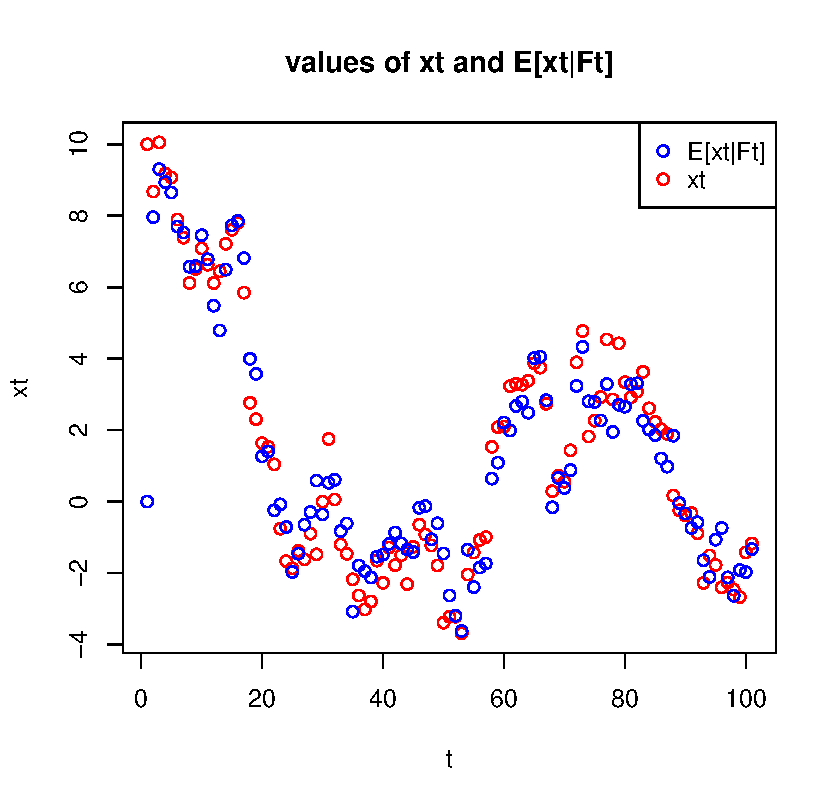
\includegraphics[height=3in,width=3in]{xt_vs_E.pdf}
\end{center}
\subsection*{5.}
For the 119 stocks, the calculations were pretty unstable for me in python, so I picked randomly 5 stocks ['AAPL','ADSK','GRMN','ALGN','ETN'] and ran the experiments on these. I calculated the returns on the stock at time $i$, the return is $R_i=\frac{X_i}{X_{i-1}}$ where $X_i$ is the price of the stock. Then I tried to solve the Markowitz problem
\begin{gather*}
    \max_{\alpha} ~~\E{\alpha^T \mu} - \frac{A}{2}\alpha^T\Sigma \alpha
\end{gather*}
The solution was derived on the lecture $\alpha^*= A^{-1}\Sigma^{-1}\mu$. \\
First I estimated $\mu$ and $\sigma$ with a rolling window of $50$, generated random portfolios and scatter plotted the returns and the volatility of the portfolios. The colormap indicates the SR and the Markowitz portfolio is denoted by red, its SP is $0.14$.

\begin{center}
    \includegraphics[width=70mm,scale=1]{images/portfolios.png}
\end{center}

After that I constructed the Markowitz portfolio with $window=[200, 300, 400, 500, 1000]$ and let the portfolios evolve in time. The results are summerized in the below plot

\begin{center}
    \includegraphics[width=70mm,scale=1]{images/returns_2.png}
\end{center}

The Sharp Ratios were 
$\{200: -0.149,~
 300: -0.109,~
 40': -0.112,~
 500: -0.0867,~
 1000: 0.0558\}$
 
 Code can be found on github : https://github.com/hbenedek/epfl-stochastic


